\documentclass[a4paper]{ctexart}
\usepackage{ctex}
\usepackage{times}
\usepackage{setspace}
\usepackage{fancyhdr}
\usepackage{graphicx}
\usepackage{wrapfig}
\usepackage{array}
\usepackage{fontspec,xunicode,xltxtra}
\usepackage{titlesec}
\usepackage{titletoc}
\usepackage[titletoc]{appendix}
\usepackage[top=30mm,bottom=30mm,left=20mm,right=20mm]{geometry}
\usepackage{enumerate}
\usepackage{caption}
\usepackage{abstract}
\setmainfont{TeX Gyre Pagella}

\captionsetup[figure]{name={图},labelsep=period,font={bf,small}}

%---------------------------------------------------------------------
%	页眉页脚设置
%---------------------------------------------------------------------
\fancypagestyle{plain}{\pagestyle{fancy}}%改变章节首页页眉
\pagestyle{fancy}
\lhead{\kaishu~面向对象程序设计/Java课程期末作业报告~}
\rhead{\kaishu~1030616134~尹达恒~}
\cfoot{\thepage}

%---------------------------------------------------------------------
%	目录页设置
%---------------------------------------------------------------------
\renewcommand{\contentsname}{\zihao{-3}{\centerline{目录}}}
\titlecontents{section}[2em]{\vspace{0.1\baselineskip}\songti\zihao{-4}}{\thecontentslabel\ }{}
{\hspace{.5em}\titlerule*[4pt]{$\cdot$}\contentspage}
\titlecontents{subsection}[4em]{\vspace{0.1\baselineskip}\songti\zihao{-4}}{\thecontentslabel\ }{}
{\hspace{.5em}\titlerule*[4pt]{$\cdot$}\contentspage}
\titlecontents{subsubsection}[6em]{\vspace{0.1\baselineskip}\songti\zihao{-4}}{\thecontentslabel\ }{}
{\hspace{.5em}\titlerule*[4pt]{$\cdot$}\contentspage}

%---------------------------------------------------------------------
%	章节编号设置
%--------------------------------------------------------------------
\ctexset {
	section = {
		number = \arabic{section},
		format = \zihao{4}\bfseries,
	},
	subsection = {
		number = \arabic{section}.\arabic{subsection},
		format = \zihao{-4}\bfseries,
	},
	subsubsection = {
		number = \arabic{section}.\arabic{subsection}.\arabic{subsubsection},
	}
}


\begin{document}
%---------------------------------------------------------------------
%	封面页
%---------------------------------------------------------------------
\begin{titlepage}
	\begin{center}
    
\includegraphics[width=0.9\textwidth]{figure//Njust.png}\\
    \vspace{10mm}
    \textbf{\zihao{2}\kaishu{物联网工程学院}}\\[0.8cm]
    \textbf{\zihao{2}\kaishu{面向对象程序设计/Java课程期末作业报告}}\\[3cm]
    \textbf{\zihao{2}\kaishu{网页端三效蒸发反应模拟程序设计}}\\[3cm]
	\vspace{\fill}
	\setlength{\extrarowheight}{3mm}
	{\songti\zihao{3}
		\begin{tabular}{rl}
			{\makebox[4\ccwd][s]{班\qquad 级:}}& ~\kaishu 物联1601\\
			{\makebox[4\ccwd][s]{姓\qquad 名:}}& ~\kaishu 尹达恒 \\ 
			{\makebox[4\ccwd][s]{学\qquad 号:}}& ~\kaishu 1030616134 \\ 
			{\makebox[4\ccwd][s]{指导老师:}} & ~\kaishu 陈树\\ 
		\end{tabular}
	}\\[2cm]
	\vspace{\fill}
	\zihao{4}
	2018\textasciitilde 2019第一学期\\
	\today
	\end{center}
\end{titlepage}

%---------------------------------------------------------------------
%  摘要
%---------------------------------------------------------------------
\renewcommand{\abstractname}{\zihao{-3}\heiti{摘要}}
\begin{spacing}{1.25}%这是段落间距
	\begin{abstract}
		\songti\zihao{-4}{三效蒸发反应广泛应用于食品、化工、医药、生物和环保领域,如牛奶、果汁、盐、糖、抗生素、氨基酸、废水的处理。由于该过程发生汽化和冷凝等相变化,蒸发过程需要消耗大量的蒸汽用于加热,装置设计、操作的优劣在很大程度上影响反应的效果。因此,如果能用计算机对三效蒸发反应进行模拟和测试,将能有效地提升三效蒸发反应器的设计和测试和维护成本,为化工厂节约大量资源。本文所介绍的三效蒸发反应模拟程序使用网页开发中常用的JavaServlet+JavaScript模式处理模拟数据,结合最近推出的高性能网页端3D图像引擎three.js进行呈现,使得对三效蒸发反应的模拟过程更加快速、结果更加直观,为三效蒸发反应器的设计和测试带来极大便利。}
		
	\end{abstract}
\end{spacing}
\newpage

%---------------------------------------------------------------------
%  目录页
%---------------------------------------------------------------------
\tableofcontents % 生成目录
\newpage

%---------------------------------------------------------------------
%  正文
%---------------------------------------------------------------------
\songti\zihao{-4}
\begin{spacing}{1.25}%这是段落间距
\section{设计要求}

\subsection{后端设计要求}
后端用Java Servlet编写,要求能接收前端发送的数据以及计算模拟结果。

\subsection{前端设计要求}\label{subsection:前端设计要求}
前端用JavaScript编写,包含以下内容:

\begin{itemize}
	\item 数据交互:能与后端进行数据交互。
	\item 三效图主体:在页面上以图像方式表现三效图模拟结果,并能根据模拟数据实时更新显示。
	\item 数据表格:在表格中以数值方式列出三效图模拟结果,并能根据模拟数据实时更新显示。
	\item 三效图参数调节滑动条:能对三效模拟的液体和气体输入进行调节。
	\item 三个按钮,功能如下:
	\begin{itemize}
		\item 开始:
		\begin{enumerate}
			\item 三效开始进料,到50\%时三效输出阀门打开,物料进入一效,同时一效蒸汽阀打开;
			\item 一效液位到达50\%时,一效输出阀门打开,物料进入二效,同时二效蒸汽阀打开;
			\item 二效液位达到50\%时,二效输出阀门打开,开始成品输出以及半成品回收。
		\end{enumerate}
	\item 保存:将当前三效模拟数据以文本文件方式保存在本地。
	\item 读取:从保存的三效模拟数据文件中读取三效模拟数据并更新模拟过程。
	\end{itemize}
\end{itemize}

\newpage
\section{设计内容}
\subsection{后端设计内容}
后端数据交互步骤如下:

\begin{enumerate}
	\item post方式接收前端传来的数据,并从中读取液体输入速率liq\_in、气体输入速率gas\_in、液位限制hMax、压强限制pMax、液体输入速率限制vlMax、气体输入速率限制vpMax;
	\begin{figure}[htbp]
		\centering
		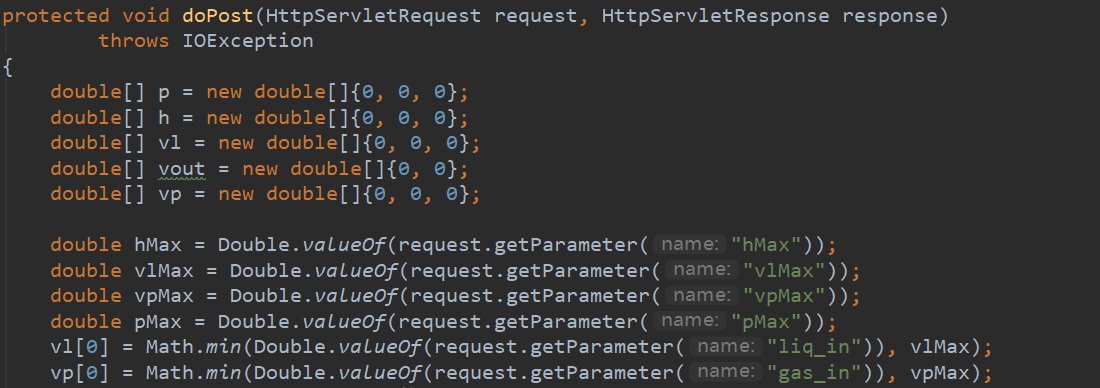
\includegraphics [width=0.75\textwidth]{figure//back1.png}
		\caption{后端程序截图:接收数据}
	\end{figure}
	\item 根据接收到的数据计算三效图各环节的模拟结果;
	\begin{figure}[htbp]
		\centering
		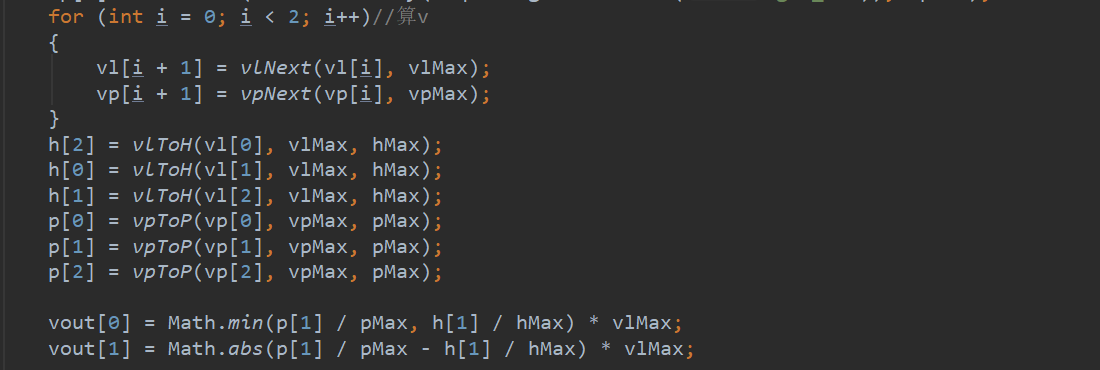
\includegraphics [width=0.75\textwidth]{figure//back2.png}
		\caption{后端程序截图:处理数据}
	\end{figure}
	\item 以JSON格式返回计算结果。
	\begin{figure}[htbp]
		\centering
		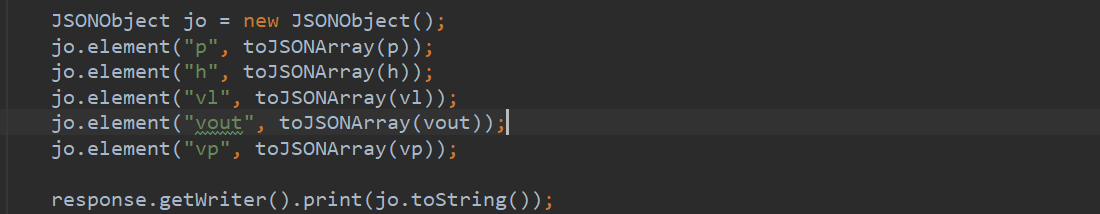
\includegraphics [width=0.75\textwidth]{figure//back3.png}
		\caption{后端程序截图:返回结果}
	\end{figure}
\end{enumerate}

\subsection{前端设计内容}
\subsubsection{前端JavaScript第三方库文件}
本项目使用的JavaScript库包括:

\begin{itemize}
	\item jQuery插件
	\item 基于WebGL图像引擎的3D渲染库three.js
	\item js文件保存插件FileSaver.js
\end{itemize}

引入的库文件的方式遵循jQuery插件和three.js库的官方文档。
\begin{figure}[htbp]
	\centering
	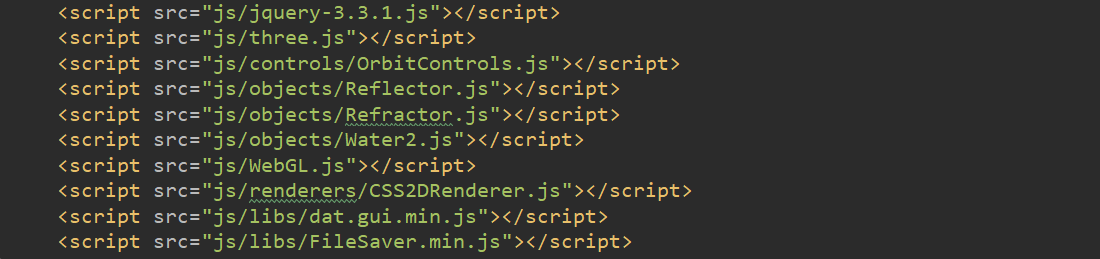
\includegraphics [width=0.8\textwidth]{figure//forw1.png}
	\caption{前端程序截图:前端所用的JavaScript第三方库文件}
\end{figure}

\subsubsection{前端JavaScript程序文件及函数功能}
前端所用的JavaScript程序文件如下图:
\begin{figure}[htbp]
	\centering
	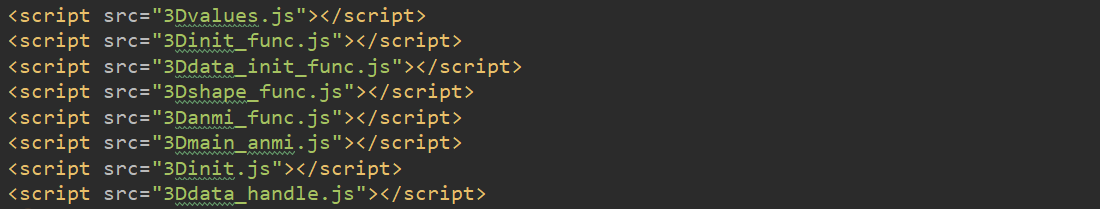
\includegraphics [width=0.8\textwidth]{figure//forw2.png}
	\caption{前端程序截图:前端所用的JavaScript程序文件}
\end{figure}

程序文件功能及其中各函数功能如下:
\begin{itemize}
	\item 3Dvalues.js:记录了绘制3D图形所需的必要信息。
	\item 3Dinit\_func.js:定义了初始化三效图时要调用的函数和初始数据,包括:
	\begin{itemize}
		\item sceneInit():初始化3D场景并添加地板平面和3D背景。
		\item lightInit():在场景中设置灯光。
		\item shapeInit():向场景中添加三效图的3D图形并贴图。
		\item rendererInit():设置并开启渲染器。
		\item cameraInit():添加并调整相机视角。
	\end{itemize}
	\item 3Ddata\_init\_func.js:定义了和后台进行数据交互时要调用的函数和初始数据,包括:
	\begin{itemize}
		\item guiInit():初始化液体和气体输入参数调节面板。
		\item requestData():向后端发送液体和气体输入数据,将返回的计算结果传入updateData(response)进行处理。
		\item updateData(response):依照传入计算结果response中的数据对前端暂存的三效模拟数据更新。
		\item start\_click():\ref{subsection:前端设计要求}中所述的“开始”按钮的点击事件所绑定的函数,更新页面显示并调用start\_anmiate()播放\ref{subsection:前端设计要求}中所描述的开始动画。
	\end{itemize}
	\item 3Dshape\_func.js:定义了用于创建3D形状的函数,这些函数会于初始化三效图时被3Dinit\_func.js中定义的shapeInit()函数调用,包括:
	\begin{itemize}
		\item createIOarrow(name):返回一个带有字符串标签的白色圆锥体,标签中的字符串为传入参数name;圆锥体的贴图不受光照影响。返回的圆锥体会被调整到液体或气体输入管道入口或产品输出口处。
		\item createBucket(name):返回一个带有字符串标签的蓝色框架型圆柱体,标签中的字符串为传入参数name。返回的圆柱体即是三效图中的反应釜。
		\item createBucketWater():返回一个由蓝色半透明圆柱体和位于圆柱体上表面的水面反射效果平面组成的3D图形组。返回的3D图形组即是三效图中反应釜里的液体,图形组会被调整到与某个反应釜在中轴线重合。
		\item calculateCurve(t, length, points):返回一个三元组,其值为点集points(四维数组)中各点顺序相连所构成的曲线上某点的坐标。传入参数中length指定了points构成的曲线长度,t(0$\leq$t$\leq$1)指定了要计算的点在曲线上的位置。此函数只在calculateTubeShape(points)中被调用。
		\item calculateTubeShape(points):返回无材质曲线管道,曲线管道的中轴线为将点集points(四维数组)中各点顺序相连所构成的曲线。此函数只在createTube(points)中被调用。
		\item createTube(points):返回蓝色框架型曲线管道,此管道为在calculateTubeShape(points)返回的无材质曲线管道上生成蓝色框架贴图而成。返回的管道框架组即是三效图中的液体管道或气体管道。
		\item createTubeWater(points, v\_water):返回曲线管道形流体,此流体为在calculateTubeShape(points)返回的无材质曲线管道上生成水面反射效果贴图而成。返回的流体即是三效图液体管道中流动的液体。v\_water指定了水面反射效果中的水体流动速度。
	\end{itemize}
	\item 3Danmi\_func.js:定义了用于在场景动画中按照模拟得到的数据更新三效图和数据表格的函数,包括:
	\begin{itemize}
		\item updateScene():调用updateHP(h,p)、updateCubeWater(vl, vout)、updateInfo(vp, vl, vout)根据前端暂存的数据更新界面显示。此函数主要在动画子进程函数animate()中调用。
		\item updateHP(h,p):更新三效图反应釜中的液位高度和压强。
		\item updateCubeWater(vl, vout):更新三效图管道中的气体或液体流动速度。
		\item updateInfo(vp, vl, vout):更新页面上数据表格里的数据。
	\end{itemize}
	\item 3Dmain\_anmi.js:定义了场景动画的两个主要函数,包括:
	\begin{itemize}
		\item animate():场景动画子进程,循环调用自身。在函数体中调用updateScene()更新界面显示。
		\item start\_anmiate():播放\ref{subsection:前端设计要求}中所描述的开始动画。只在start\_click()函数中被调用。
	\end{itemize}
	\item 3Dinit.js:调用上述文件中的函数执行页面初始化操作。
	\item 3Ddata\_handle.js:定义了用于保存数据文件和读取数据文件的函数,包括:
	\begin{itemize}
		\item handleFiles(files):传入参数files为上传的数据文件,读取文件中的信息并更新显示。
		\item saveData():将当前数据保存为JSON格式的文本文件。
	\end{itemize}
\end{itemize}

\subsubsection{三效图初始化过程}
\begin{enumerate}
	\item 3Dvalues.js中定义并初始化所有3D图形的大小和位置数组。
	\item 3Dmain\_anmi.js中调用sceneInit()初始化3D场景。
	\item 3Dmain\_anmi.js中调用lightInit()初始化灯光。
	\item 3Dmain\_anmi.js中调用shapeInit()初始化三效图的形状和贴图。
	\item 3Dmain\_anmi.js中调用rendererInit()设置并开启场景渲染。
	\item 3Dmain\_anmi.js中调用cameraInit()初始化视角位置和方向。
	\item 3Dmain\_anmi.js中调用animate()开启动画子进程。
\end{enumerate}

\begin{figure}[htbp]
	\centering
	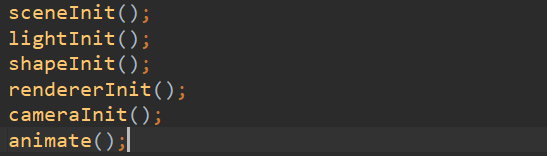
\includegraphics [width=0.8\textwidth]{figure//forw3.png}
	\caption{前端程序截图:3Dinit.js三效图初始化过程}
\end{figure}

\subsubsection{三效图动画子进程运行原理}
三效图的动画子进程animate()是独立于主进程运行的,其功能是通过不断读取前端暂存的三效模拟数据和当前显示的三效模拟效果进行比较,按照比较结果对三效图中各3D图形的参数进行更新,同时更新数据表格中显示的数值,以达到实时更新的效果。因此每当前端暂存的三效模拟数据发生变化时,动画子进程animate()中都能检测到变化并及时做出响应调整界面显示。

此外,动画子进程animate()中更新显示的函数并不是完全按照前端暂存的三效模拟数据立即更新3D图形的参数,而是按照当前显示的模拟值和暂存的三效模拟数据的差值进行适当调整,从而一定程度上模拟出实际三效蒸发反应中负反馈调节的效果。

\newpage
\section{程序运行截图}
\begin{figure}[htbp]
	\centering
	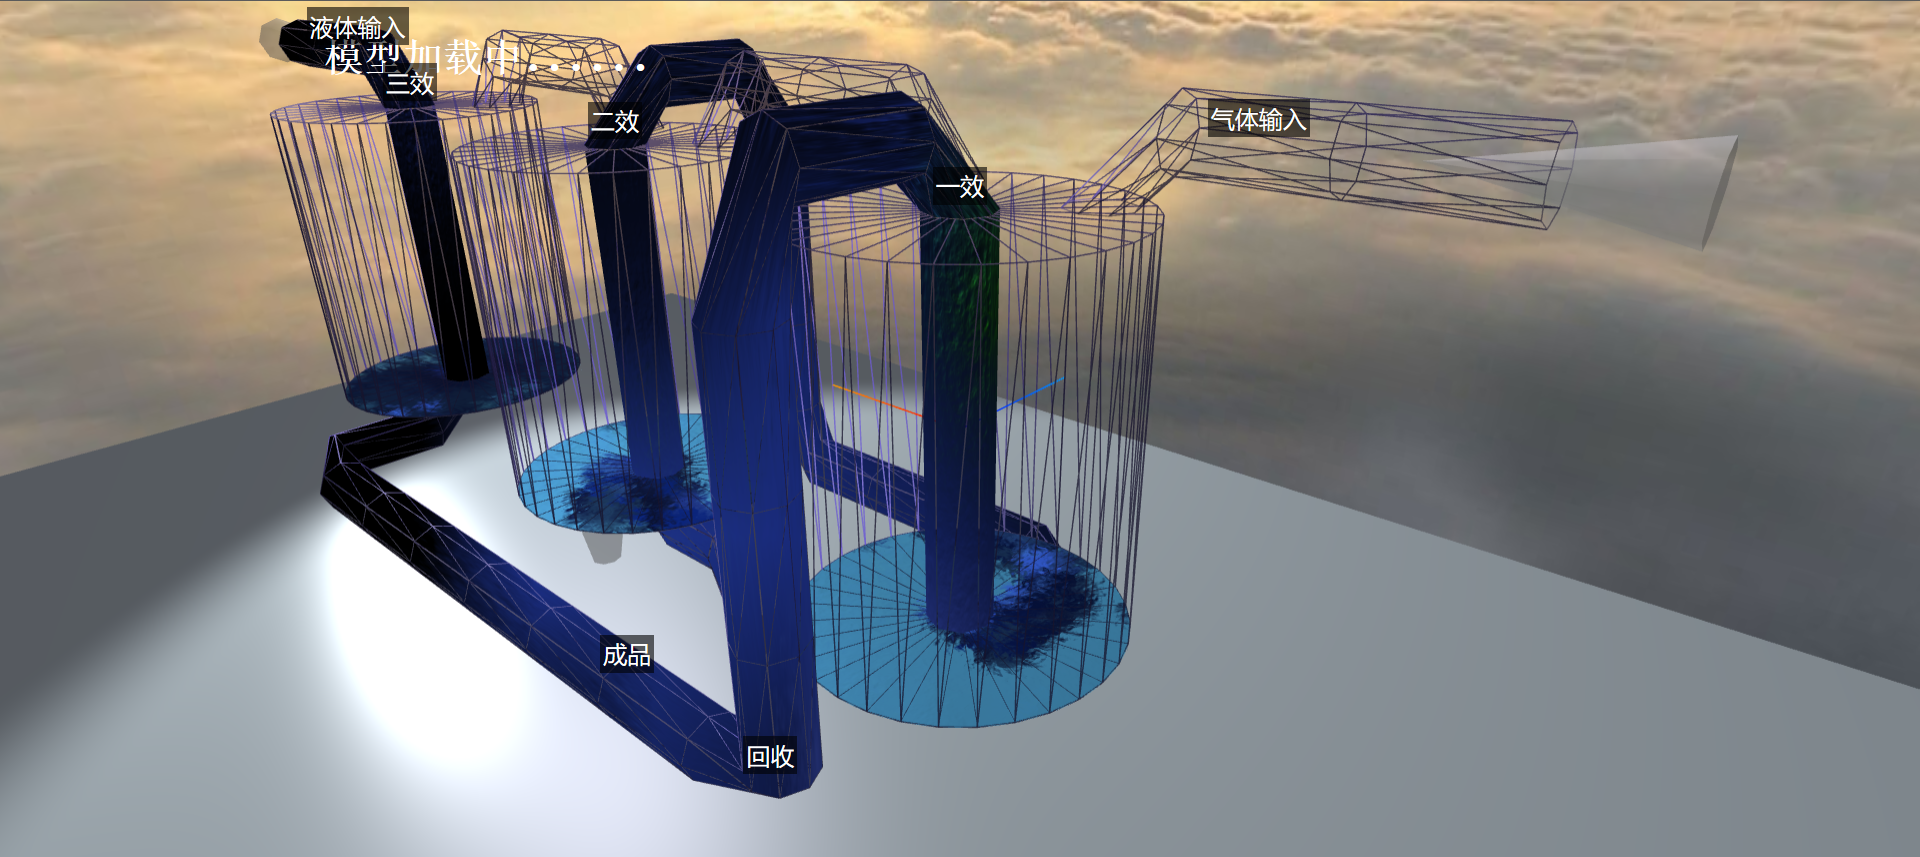
\includegraphics [width=\textwidth]{figure//res0.png}
	\caption{程序运行截图:三效图初始化}
\end{figure}
\begin{figure}[htbp]
	\centering
	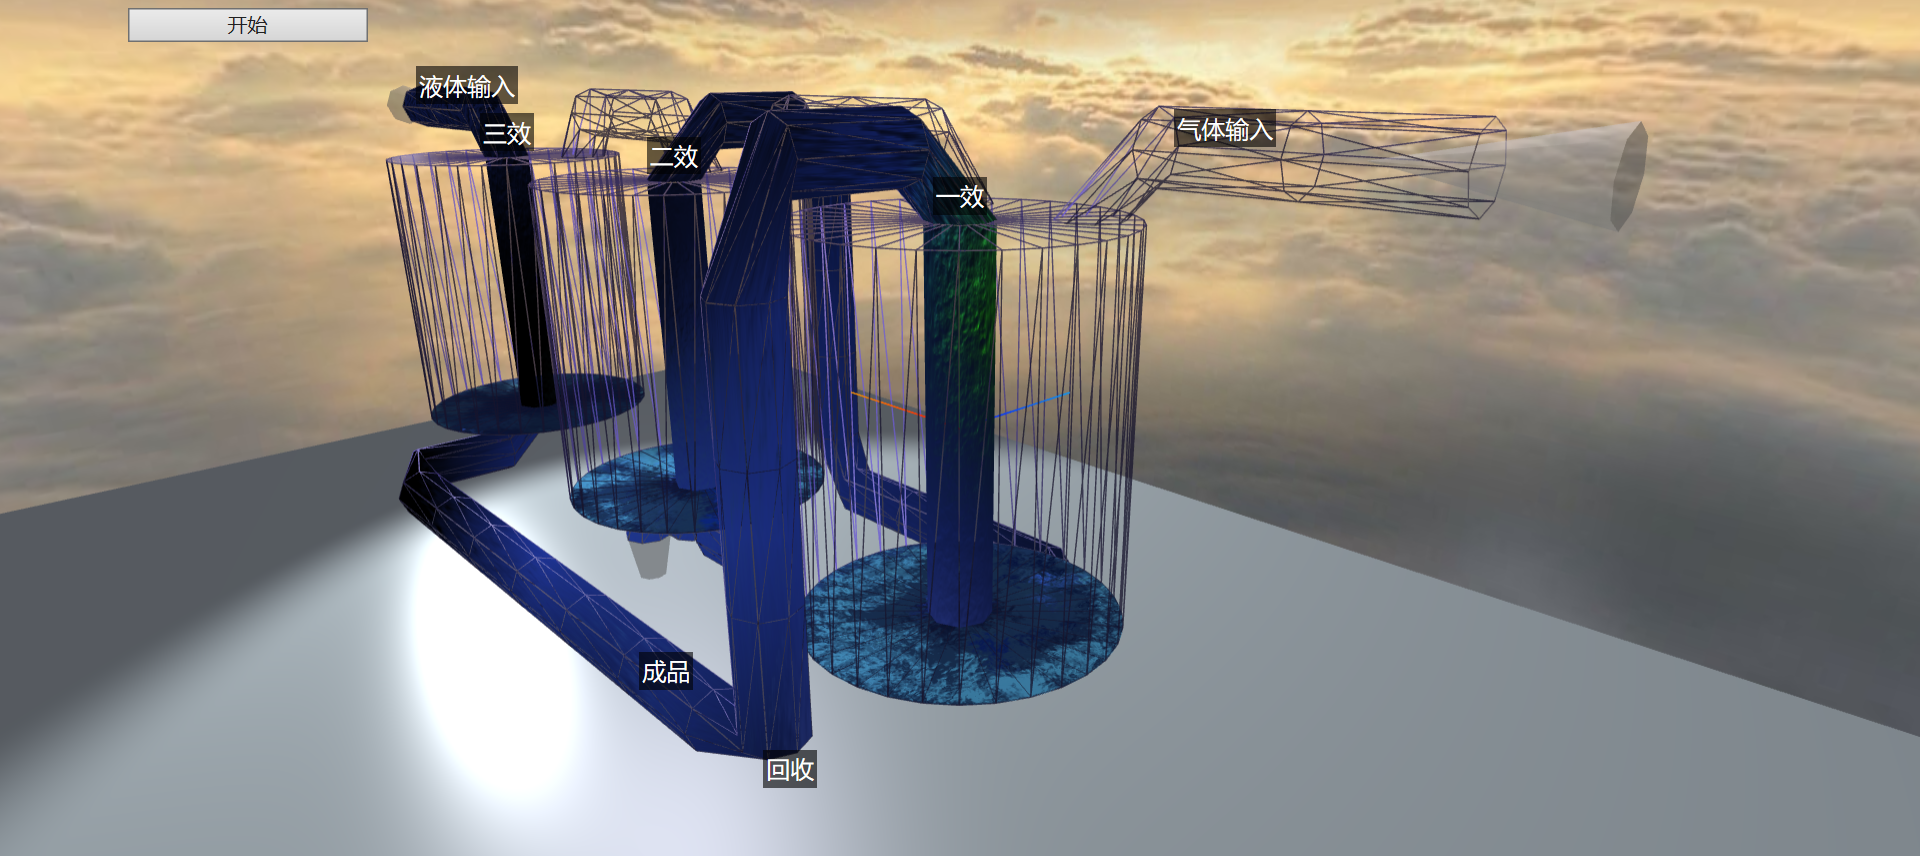
\includegraphics [width=\textwidth]{figure//res1.png}
	\caption{程序运行截图:三效图初始化完成}
\end{figure}
\begin{figure}[htbp]
	\centering
	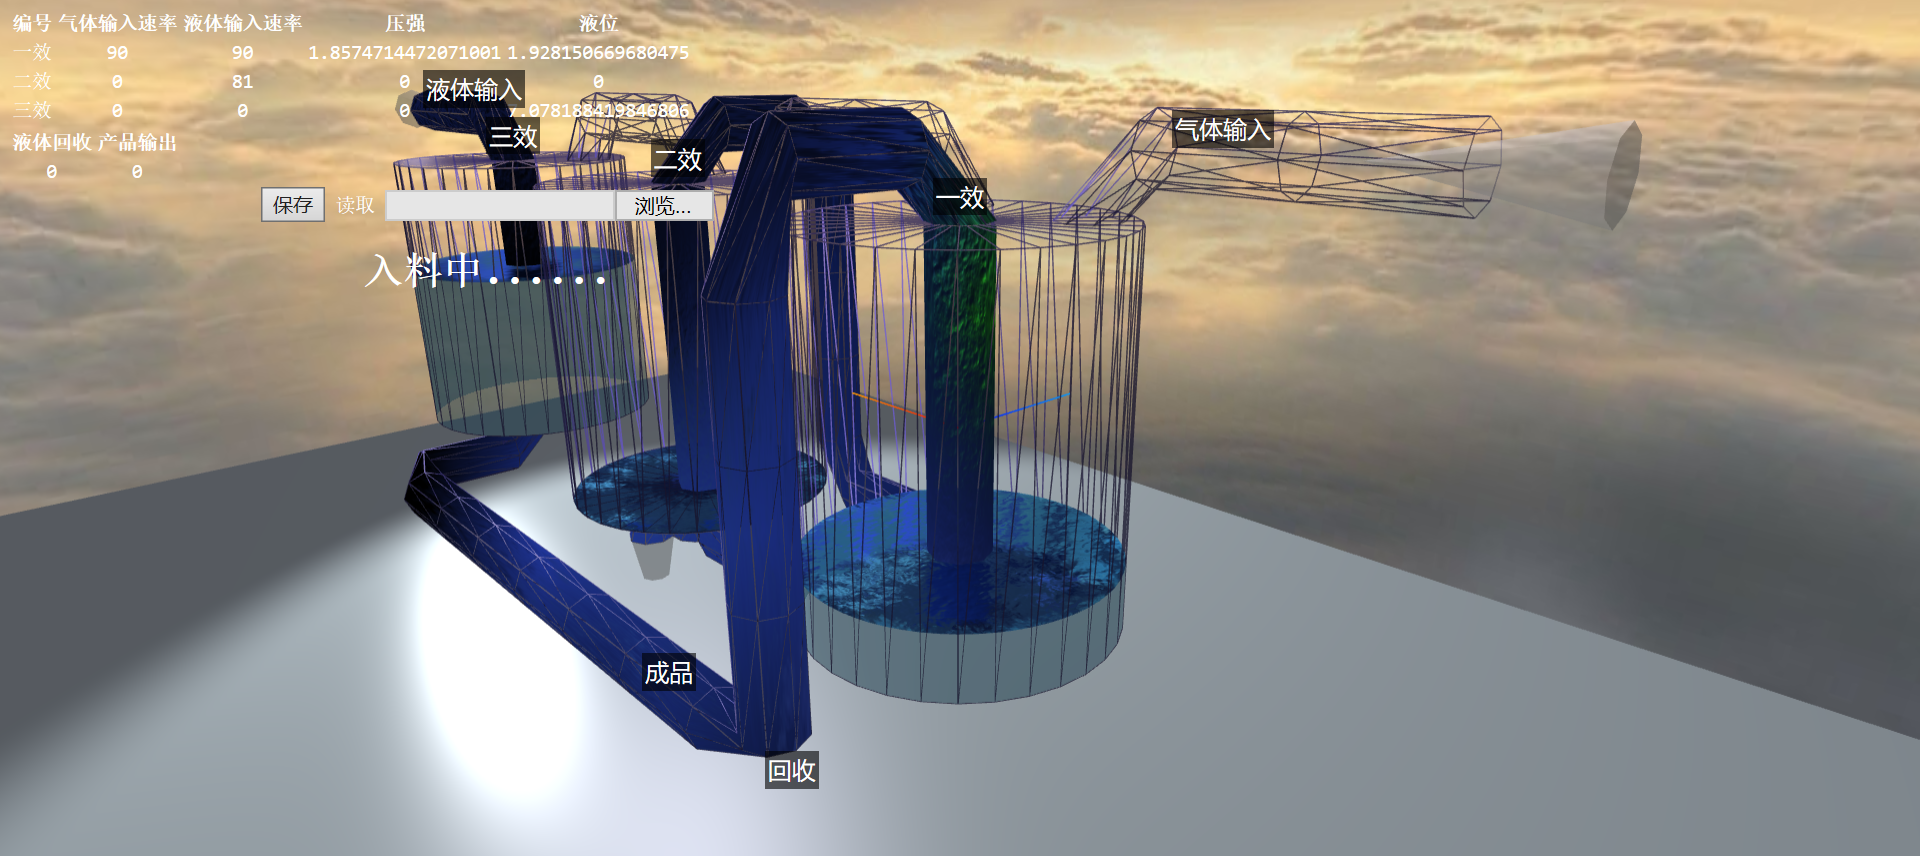
\includegraphics [width=\textwidth]{figure//res2.png}
	\caption{程序运行截图:开始入料}
\end{figure}
\begin{figure}[htbp]
	\centering
	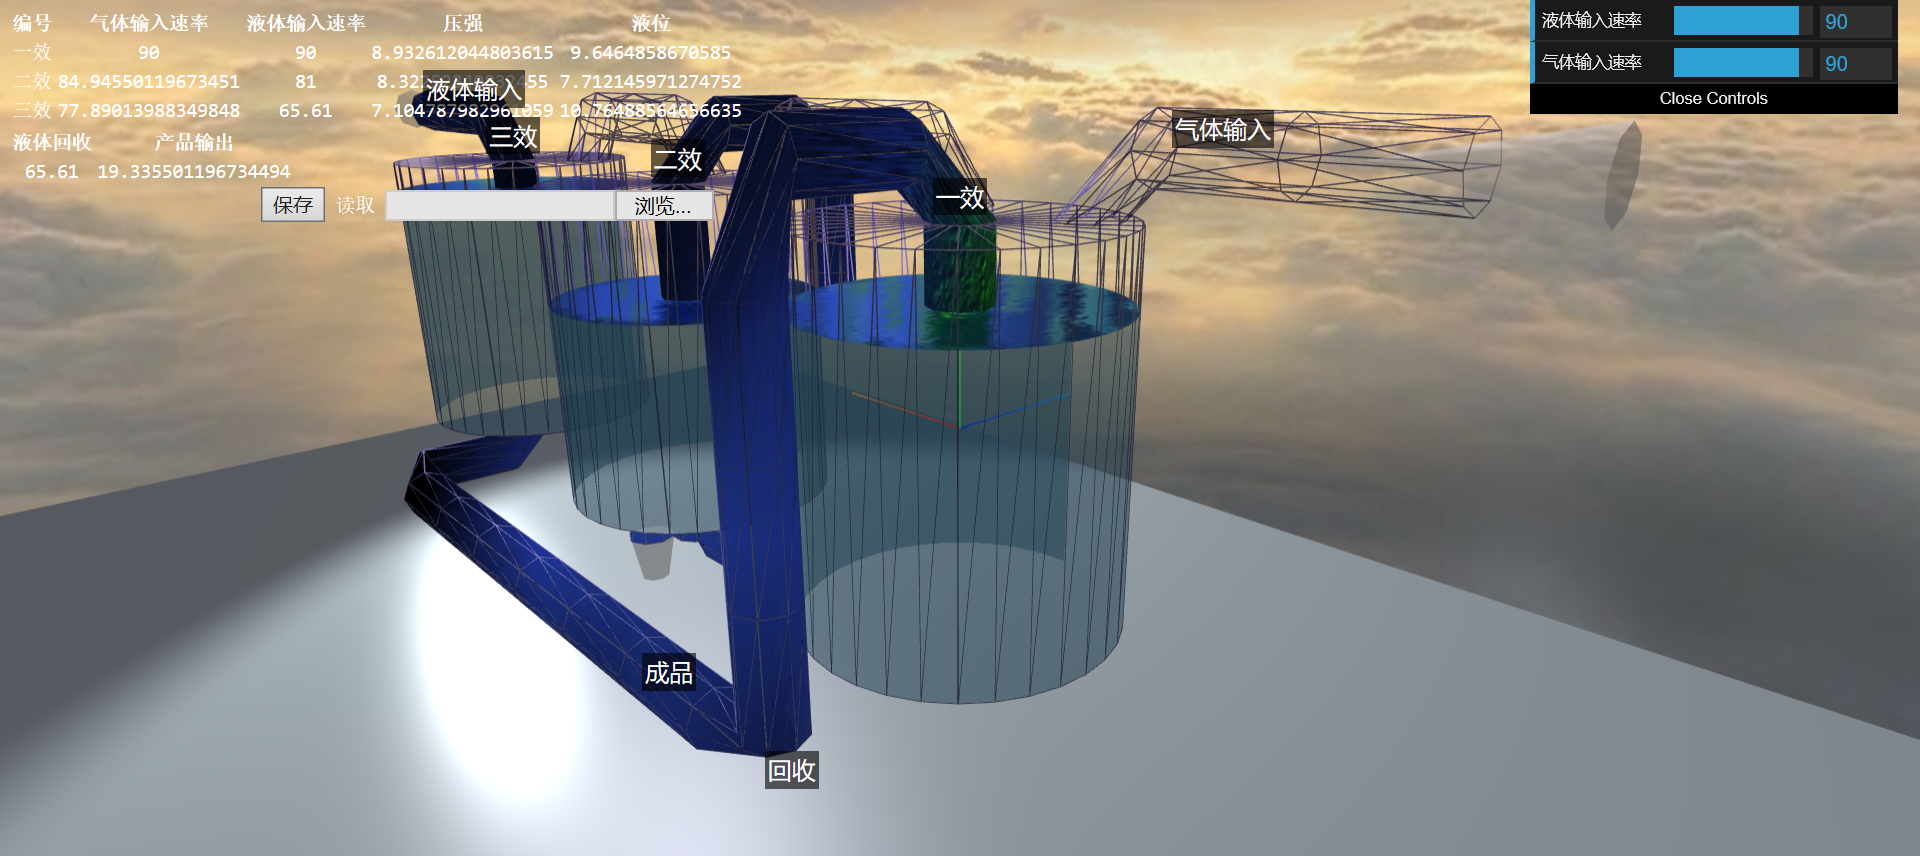
\includegraphics [width=\textwidth]{figure//res3.png}
	\caption{程序运行截图:入料完成}
\end{figure}
\begin{figure}[htbp]
	\centering
	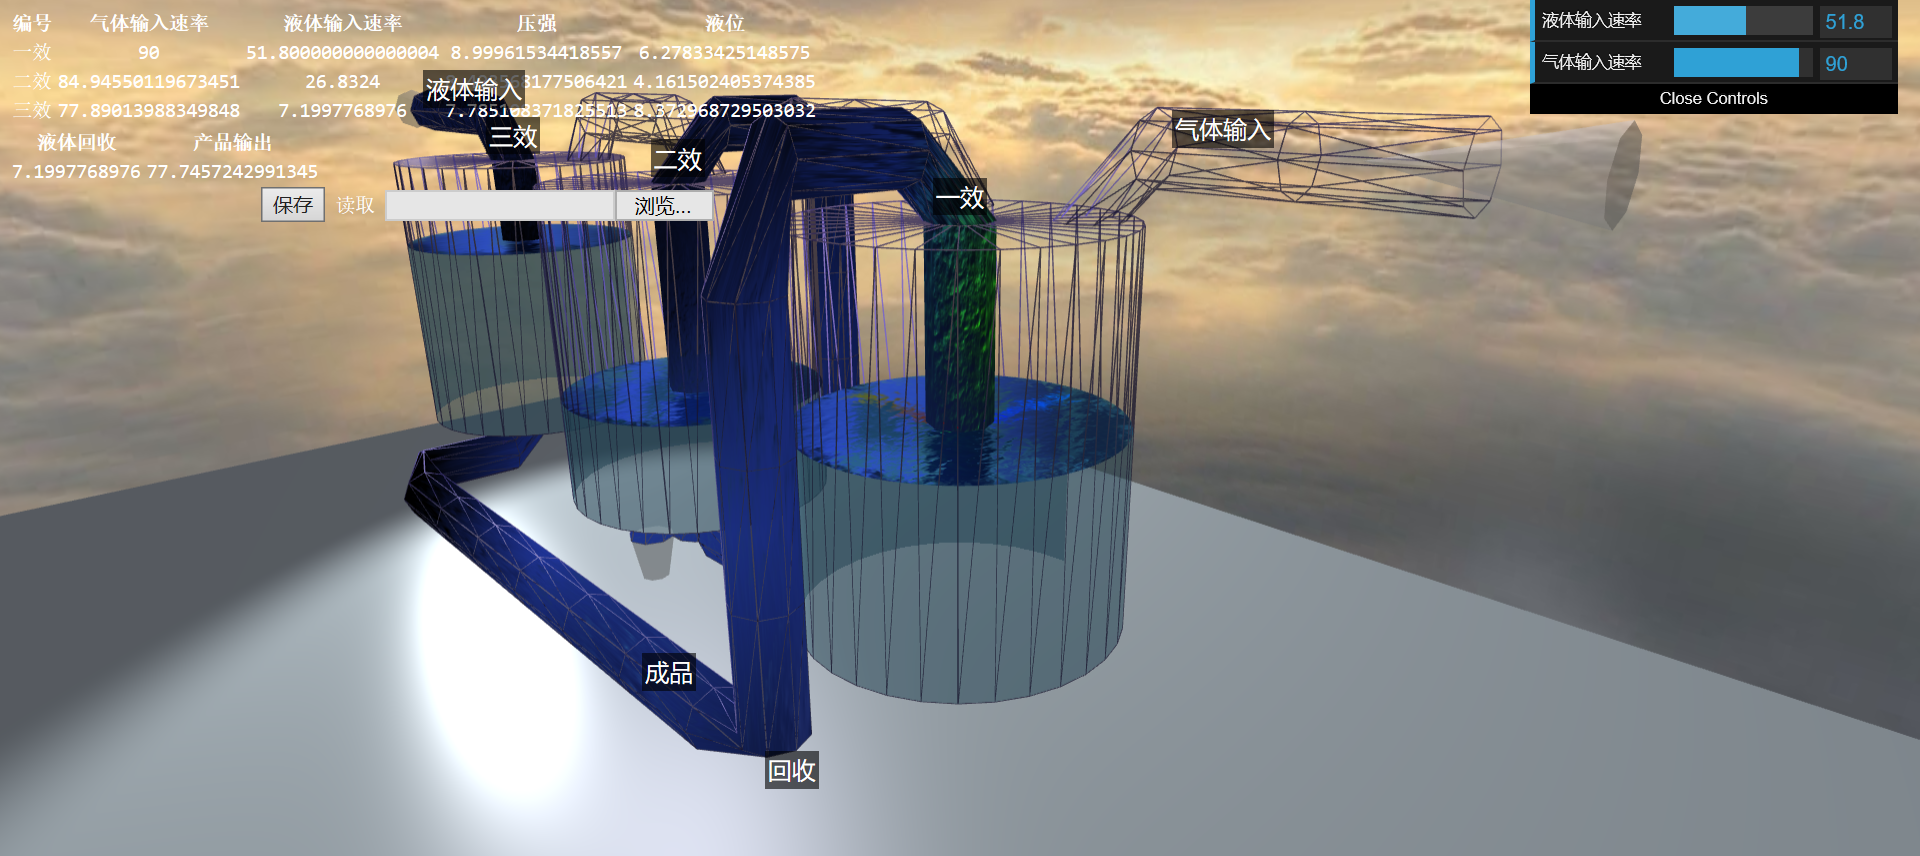
\includegraphics [width=\textwidth]{figure//res4.png}
	\caption{程序运行截图:调整液体输入速率}
\end{figure}
\begin{figure}[htbp]
	\centering
	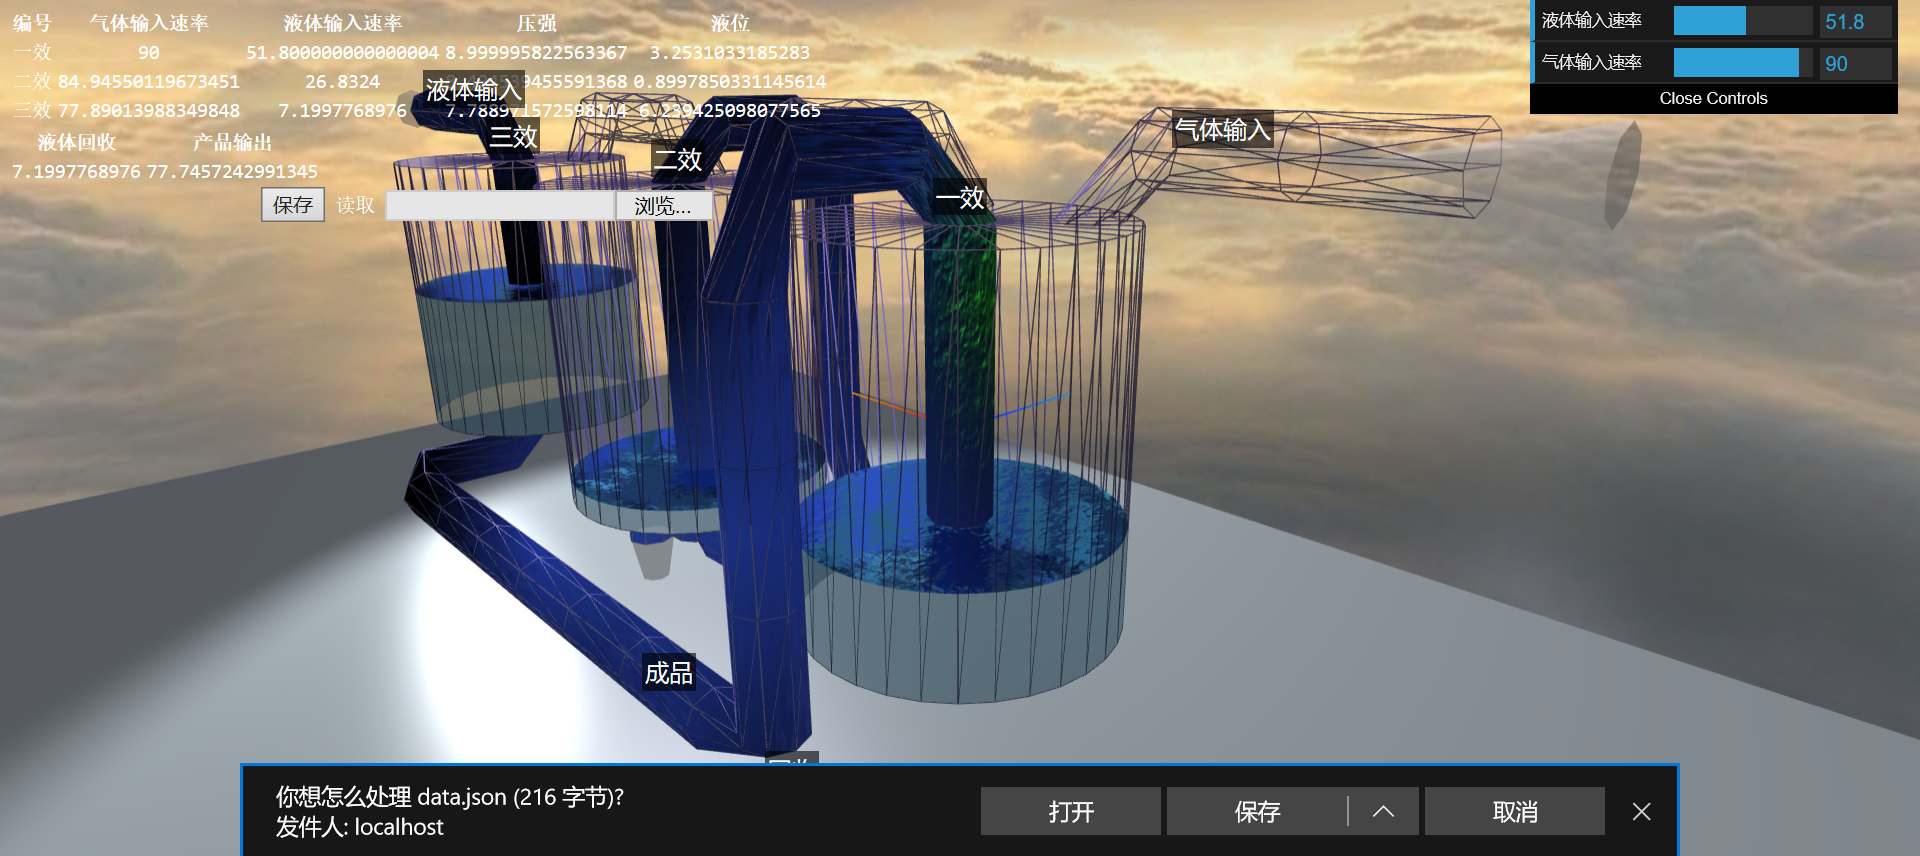
\includegraphics [width=\textwidth]{figure//res5.png}
	\caption{程序运行截图:保存数据文件}
\end{figure}
\begin{figure}[htbp]
	\centering
	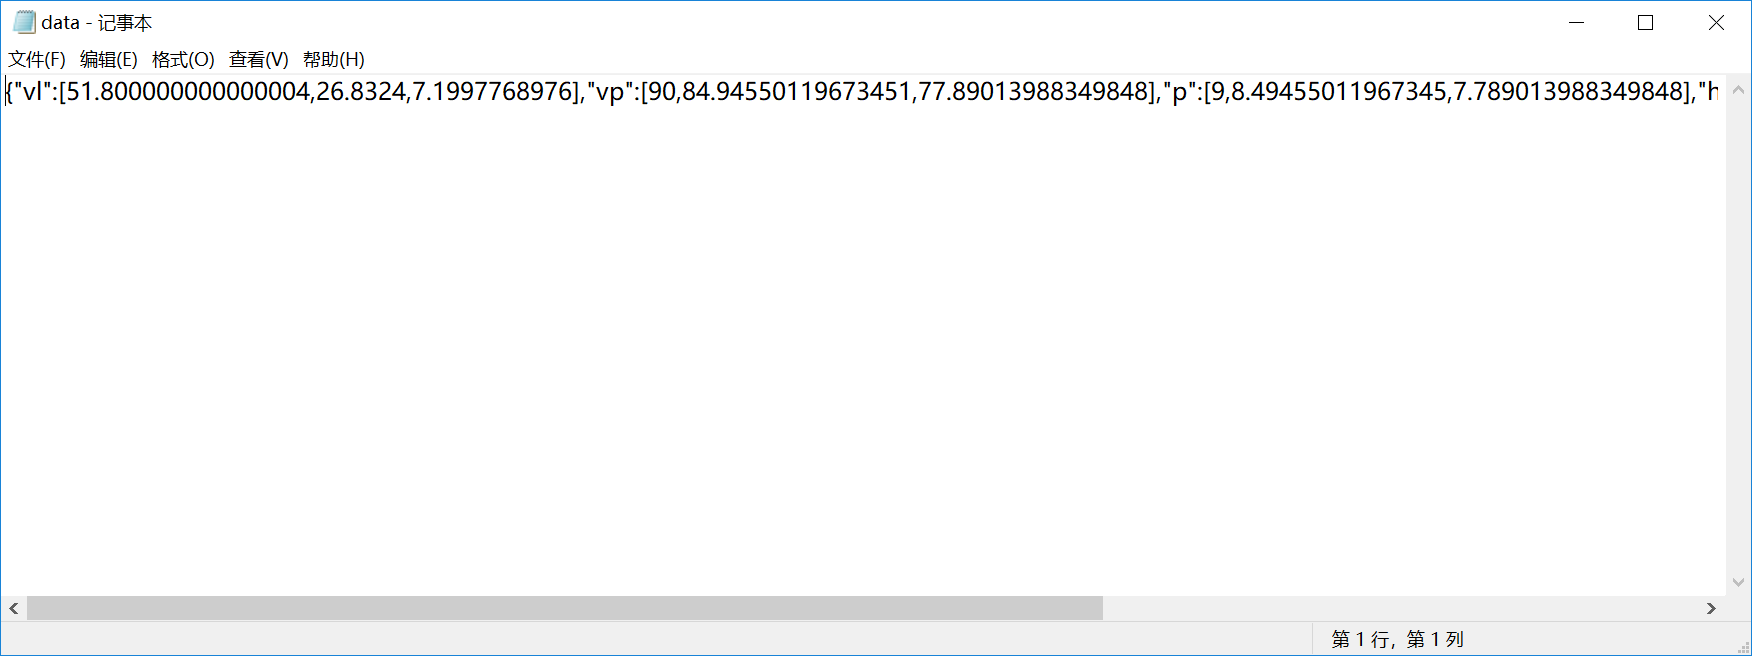
\includegraphics [width=\textwidth]{figure//res6.png}
	\caption{程序运行截图:数据文件格式}
\end{figure}
\begin{figure}[htbp]
	\centering
	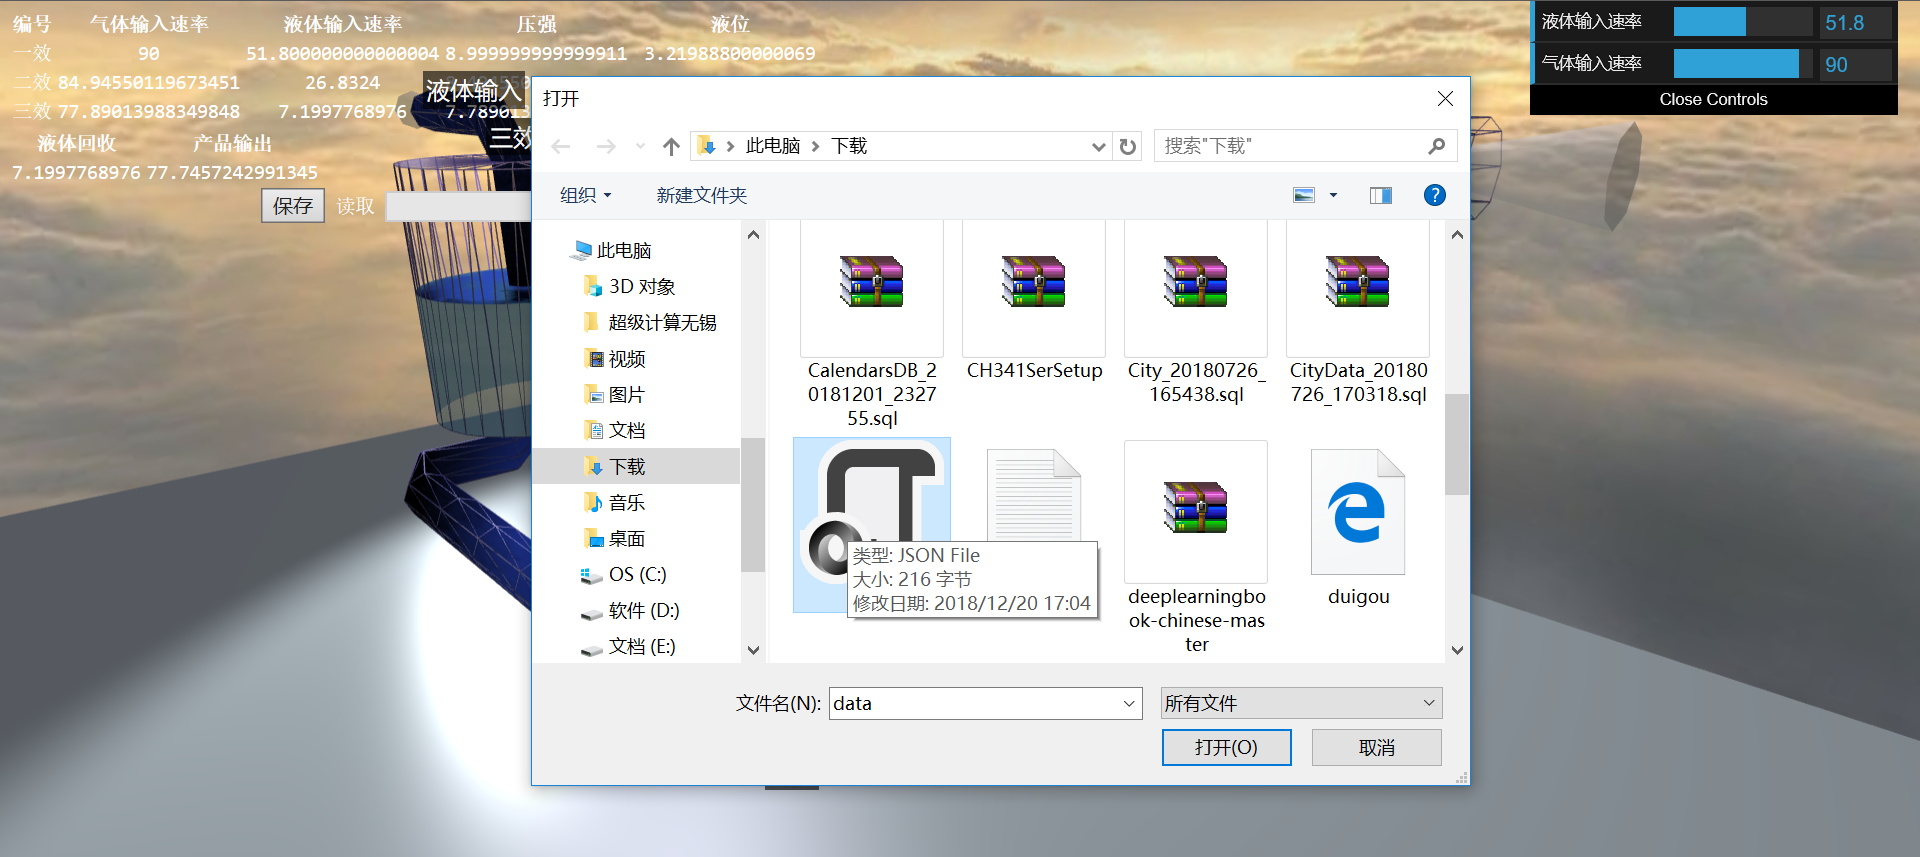
\includegraphics [width=\textwidth]{figure//res7.png}
	\caption{程序运行截图:读取数据文件}
\end{figure}
\end{spacing}
\end{document}